\documentclass[12pt]{article}
\usepackage[margin=1in]{geometry}
\usepackage{fancyvrb}
\usepackage{multicol}
\usepackage{hyperref}
\usepackage{amsmath}
\usepackage{amsfonts}

\usepackage[listings]{tcolorbox}

\definecolor{codegreen}{rgb}{0,0.6,0}
\definecolor{codegray}{rgb}{0.5,0.5,0.5}
\definecolor{codepurple}{rgb}{0.58,0,0.82}
\definecolor{backcolour}{rgb}{0.95,0.95,0.92}

\lstdefinestyle{mystyle}{
    language=Python,
    backgroundcolor=\color{backcolour},   
    commentstyle=\color{codegreen},
    keywordstyle=\color{magenta},
    numberstyle=\tiny\color{codegray},
    stringstyle=\color{codepurple},
    basicstyle=\ttfamily\footnotesize,
    breakatwhitespace=false,         
    breaklines=true,                 
    captionpos=b,                    
    keepspaces=true,                 
    numbers=left,                    
    numbersep=5pt,                  
    showspaces=false,                
    showstringspaces=false,
    showtabs=false,                  
    tabsize=2,
    escapechar=|,
    frame=single
}

\lstset{style=mystyle}

\newcommand{\showfig}[2]{
\noindent\includegraphics[width=\textwidth]{#1}
\centerline{#1}
}

\begin{document}
\sloppy
\pagenumbering{gobble}
\centerline{\Large CSCI 111, Bonus Lab 5}
\centerline{\large Penrose Turtle }

\centerline{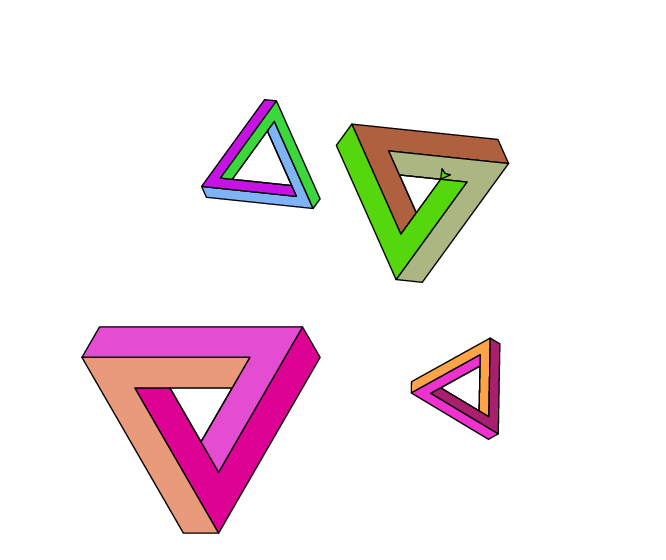
\includegraphics[scale=0.75]{penrose}}

\begin{description}


\item[Individual work:]  All work must be your own.  Do not share
code with anyone other than the instructor and teaching assistants.
This includes looking over shoulders at screens with the code open.
You may discuss ideas, algorithms, approaches, {\em etc.} with
other students but NEVER actual code.

\item[Penrose triangle:]  Described as the essence of paradox,
the Penrose triangle, seen above, is a favorite of mine.
Write a program using turtle graphics to make a Penrose
triangle.

The drawing consists of three identical shapes, each of which
can have a different fill color.  Also, the sizes of the hole
and the width of the bar should be parameters.  Finally,
whether to do a left twist or a right one should be
provided as a boolean.  So,
the main routine should look like this:
\begin{lstlisting}
def penrose(hole_size, bar_size, left_twist, colors):
    for i in range(3):
        penrose_arm(hole_size, bar_size, left_twist, colors[i])
\end{lstlisting}
where colors is an array of colors in turtle graphics
format.

The current position and orientation of the turtle
will determine where and at what angle the triangle is drawn.

The final position and orientation of the turtle after each
arm should be ready for the next arm.  The turtle will thus
end up right where it started at the end (ready to draw the
first arm again).


\end{description}

\end{document}
